\section{Data}\label{sec:data}

The dataset consists of images captured using a scanning electron microscope (SEM). As said before these images are part of a study focused on the thickness of coating cladding layers applied to various materials. In Figure~\ref{fig:three-images}, the coating layers are shown in cropped SEM images. The right side of each image highlights the coating layer with a red border, while the left side shows the original, unmarked region for comparison. 
%shrink to 4 pixels

\begin{figure}[H]
    \centering


    % First image
    \begin{subfigure}{0.8\textwidth}
        \centering
        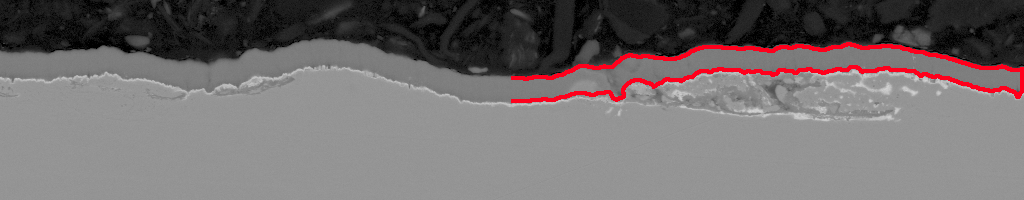
\includegraphics[width=\linewidth]{PICTURES/original_data/11_crop.png}
        \label{fig:subfig1}
    \end{subfigure}

    \vspace{0.5em}

    % Second image
    \begin{subfigure}{0.8\textwidth}
        \centering
        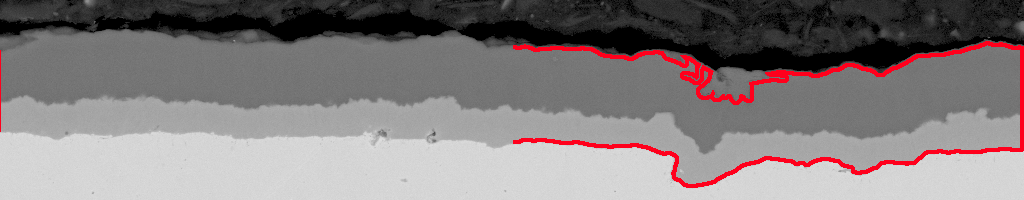
\includegraphics[width=\linewidth]{PICTURES/original_data/177_crop.png}
        \label{fig:subfig2}
    \end{subfigure}

    \vspace{0.5em}

    % Third image
    \begin{subfigure}{0.8\textwidth}
        \centering
        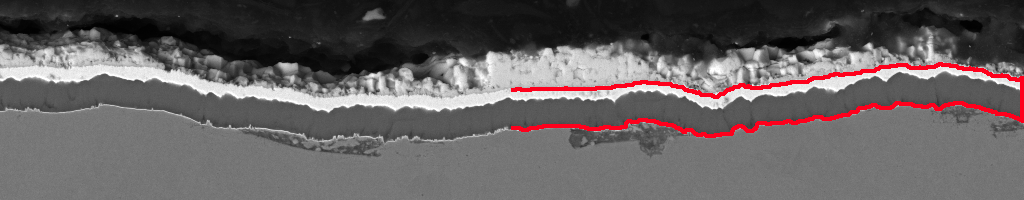
\includegraphics[width=\linewidth]{PICTURES/original_data/208_crop.png}
        \label{fig:subfig3}
    \end{subfigure}

    \caption{Cropped SEM images with partially highlighted coating layers with red border.}
    \label{fig:three-images}
    \end{figure}

The material beneath the coating in the samples varies, and the applied coating layers differ in both composition and physical characteristics. Variations are often observed at the interface between the coating and the underlying material, as well as along the top surface, where signs of oxidation may appear. Additionally, surface damage—such as fractures in the coating layer—is commonly present. These factors complicate the task of clearly identifying where the coating begins and ends, as the visual boundaries are not always well-defined. As a result, manual labeling becomes a time-consuming process.


\subsection{Manual Data Processing}\label{sec:ManualProc}

The images are initially obtained in *.tif format after the measurements with the SEM. Then they are processed using Fiji, an open-source image processing software that is a distribution of ImageJ \cite{Schindelin2012}. A predefined template consisting of 20 lines is used for measurements, each corresponding to a specific measurement region. The first ten expert-made measurements, indexed 1 to 10, are employed to measure the thickness of the coating layer, while the second set of ten lines, located beneath the first, is used to measure oxidation, which is not that common for images with coating layer. The lines are evenly distributed across the image's width and share a constant x-coordinate. The choice of ten lines was a compromise between accuracy and efficiency—while using more lines could improve precision, ten provided a good balance between informative value and the time required for manual adjustment.

Subsequent to the initial measurements, each of the 20 lines is manually adjusted to align with either the oxidation or the coating layer. After all adjustments are completed, the length of each line is exported to Excel for statistical analysis. If a layer is absent at the location of a predefined line, the line is left in its position but is later marked as 0.0 in the corresponding Excel spreadsheet.


% As a result, the researcher obtained Excel data and images, which were insufficient to form a complete dataset. Therefore, two possible solutions were considered: either to try an unsupervised method that does not require masks or to create a new dataset with masks. As will be discussed later in Section~\ref{sec:kmeans}, the unsupervised approach did not provide good results. This outcome highlighted the necessity of masks and led to the adjustments made in Fiji, described in Section~\ref{sec:1.2.2}.

The images are grouped into sets of approximately 30, with each set containing images of the same material. Different parts of the same material are captured in each set, leading to high similarity among the images in each set. The initial image of each set typically takes longer to process since the line adjustments from the previous image are reused for the other images in the same set. As the remaining images within a set are more similar, they require less time for adjustment. The primary challenges arise in images with significant oxidation, which may destroy the coating layer.

Figure~\ref{fig:Fiji} illustrates the measurements performed in Fiji. Lines 1 to 10, used for measuring the coating layer, are shown. In this example, no oxidation layer is present.

\begin{figure}[H]
    \centering
    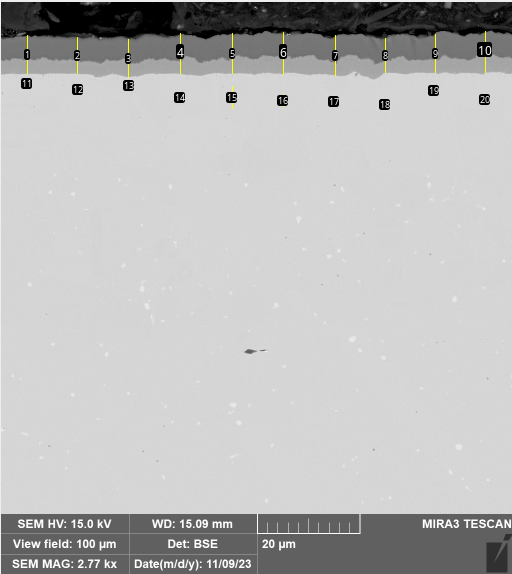
\includegraphics[width=0.7\linewidth]{PICTURES/625_Al2O3_3500h_low_cross_strana2_13_measurements.png}
    \caption{Measurement in Fiji software.}
    \label{fig:Fiji}
\end{figure}


Although oxidation and coating layers are both critical for material characterization, this thesis focuses specifically on automating the measurement of coating layer thickness in SEM images. Coating layers prevent underlying materials from oxidizing, making oxidation layers less common in samples that feature coatings.

